% Created by tikzDevice version 0.8.1 on 2015-05-25 07:37:28
% !TEX encoding = UTF-8 Unicode
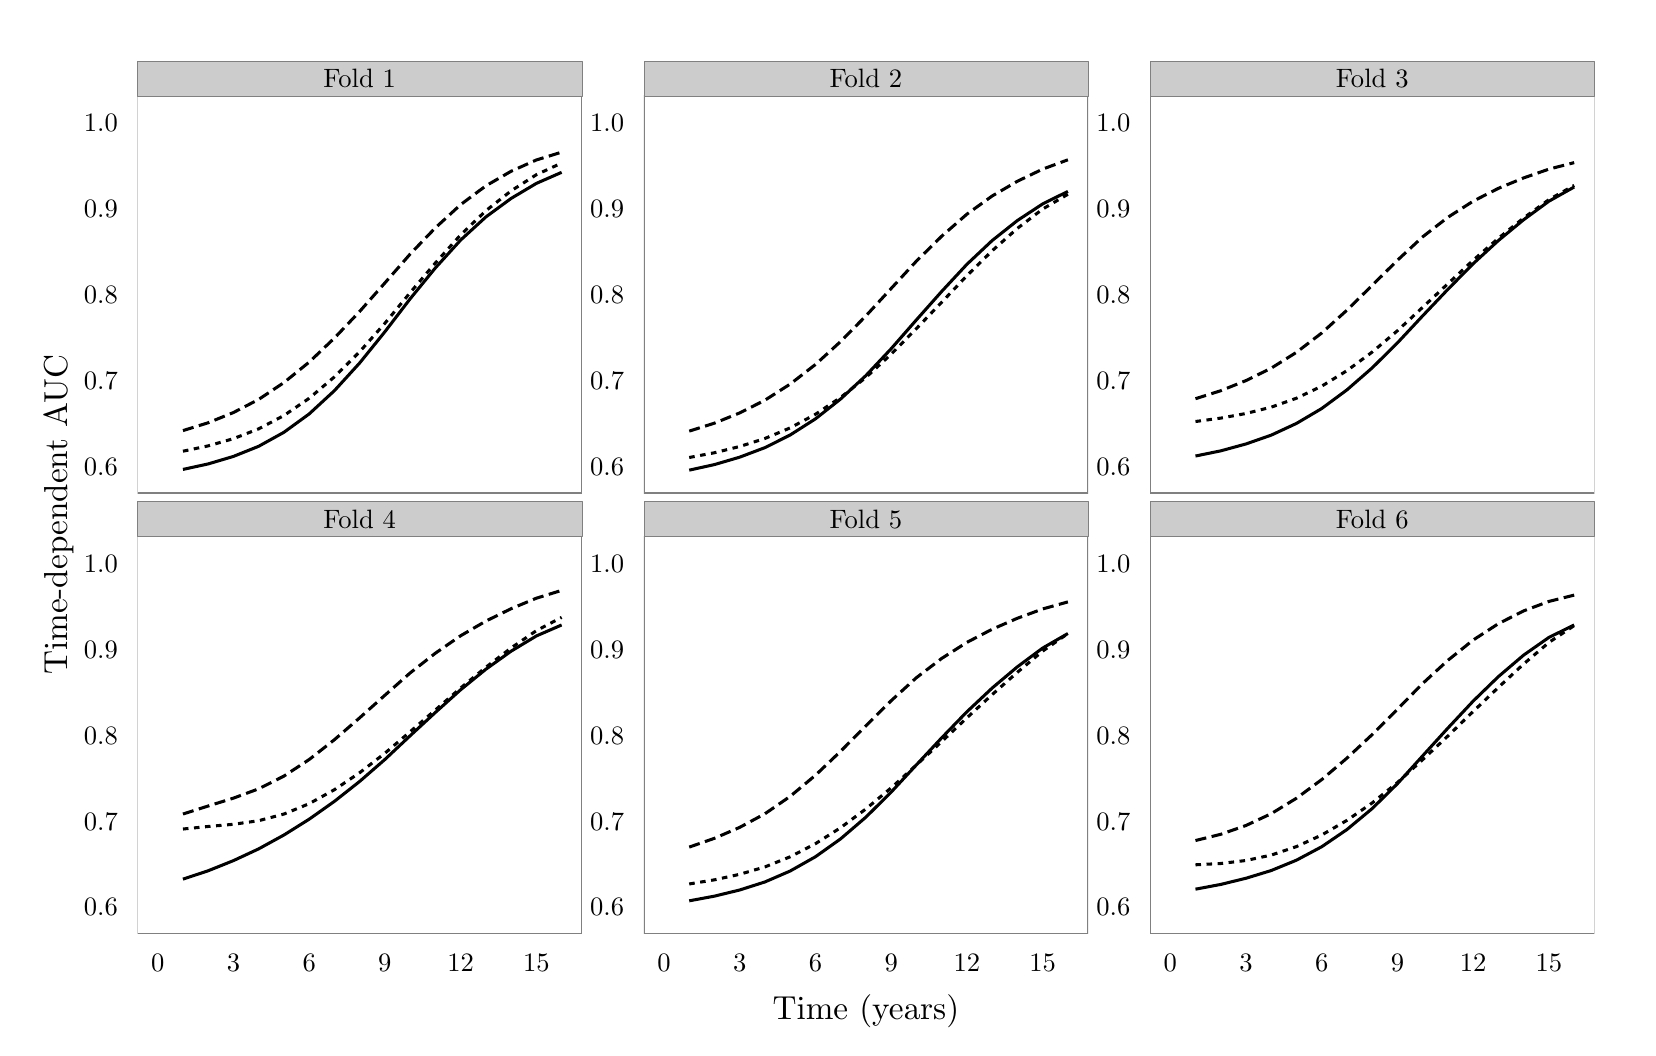
\begin{tikzpicture}[x=1pt,y=1pt]
\definecolor{fillColor}{RGB}{255,255,255}
\path[use as bounding box,fill=fillColor,fill opacity=0.00] (0,0) rectangle (578.16,361.35);
\begin{scope}
\path[clip] (  0.00,  0.00) rectangle (578.16,361.35);
\definecolor{drawColor}{RGB}{255,255,255}
\definecolor{fillColor}{RGB}{255,255,255}

\path[draw=drawColor,line width= 0.6pt,line join=round,line cap=round,fill=fillColor] ( -0.00,  0.00) rectangle (578.16,361.35);
\end{scope}
\begin{scope}
\path[clip] ( 39.69,193.18) rectangle (200.24,336.67);
\definecolor{fillColor}{RGB}{255,255,255}

\path[fill=fillColor] ( 39.69,193.18) rectangle (200.24,336.67);
\definecolor{drawColor}{RGB}{0,0,0}

\path[draw=drawColor,line width= 1.1pt,line join=round] ( 56.11,201.72) --
	( 65.23,203.71) --
	( 74.35,206.42) --
	( 83.47,210.08) --
	( 92.60,215.14) --
	(101.72,221.77) --
	(110.84,230.18) --
	(119.96,240.18) --
	(129.08,251.47) --
	(138.21,263.38) --
	(147.33,274.54) --
	(156.45,284.60) --
	(165.57,292.95) --
	(174.70,299.65) --
	(183.82,305.08) --
	(192.94,309.07);

\path[draw=drawColor,line width= 1.1pt,dash pattern=on 2pt off 2pt ,line join=round] ( 56.11,208.30) --
	( 65.23,210.23) --
	( 74.35,212.84) --
	( 83.47,216.38) --
	( 92.60,221.20) --
	(101.72,227.43) --
	(110.84,235.16) --
	(119.96,244.24) --
	(129.08,254.53) --
	(138.21,265.60) --
	(147.33,276.33) --
	(156.45,286.47) --
	(165.57,295.20) --
	(174.70,302.39) --
	(183.82,308.22) --
	(192.94,312.43);

\path[draw=drawColor,line width= 1.1pt,dash pattern=on 4pt off 2pt ,line join=round] ( 56.11,215.75) --
	( 65.23,218.58) --
	( 74.35,222.28) --
	( 83.47,227.01) --
	( 92.60,233.11) --
	(101.72,240.50) --
	(110.84,249.18) --
	(119.96,258.80) --
	(129.08,269.11) --
	(138.21,279.54) --
	(147.33,289.03) --
	(156.45,297.41) --
	(165.57,304.19) --
	(174.70,309.47) --
	(183.82,313.54) --
	(192.94,316.36);
\definecolor{drawColor}{gray}{0.50}

\path[draw=drawColor,line width= 0.6pt,line join=round,line cap=round] ( 39.69,193.18) rectangle (200.24,336.67);
\end{scope}
\begin{scope}
\path[clip] (222.63,193.18) rectangle (383.18,336.67);
\definecolor{fillColor}{RGB}{255,255,255}

\path[fill=fillColor] (222.63,193.18) rectangle (383.18,336.67);
\definecolor{drawColor}{RGB}{0,0,0}

\path[draw=drawColor,line width= 1.1pt,line join=round] (239.05,201.46) --
	(248.17,203.47) --
	(257.29,206.15) --
	(266.41,209.60) --
	(275.53,214.17) --
	(284.66,219.99) --
	(293.78,227.19) --
	(302.90,235.65) --
	(312.02,245.34) --
	(321.15,255.77) --
	(330.27,266.03) --
	(339.39,275.84) --
	(348.51,284.42) --
	(357.63,291.66) --
	(366.76,297.66) --
	(375.88,302.18);

\path[draw=drawColor,line width= 1.1pt,dash pattern=on 2pt off 2pt ,line join=round] (239.05,206.03) --
	(248.17,207.75) --
	(257.29,210.00) --
	(266.41,212.90) --
	(275.53,216.73) --
	(284.66,221.64) --
	(293.78,227.74) --
	(302.90,234.97) --
	(312.02,243.37) --
	(321.15,252.63) --
	(330.27,262.12) --
	(339.39,271.73) --
	(348.51,280.73) --
	(357.63,288.82) --
	(366.76,295.80) --
	(375.88,301.15);

\path[draw=drawColor,line width= 1.1pt,dash pattern=on 4pt off 2pt ,line join=round] (239.05,215.56) --
	(248.17,218.44) --
	(257.29,222.14) --
	(266.41,226.74) --
	(275.53,232.56) --
	(284.66,239.64) --
	(293.78,247.96) --
	(302.90,257.21) --
	(312.02,267.11) --
	(321.15,277.00) --
	(330.27,285.99) --
	(339.39,293.96) --
	(348.51,300.52) --
	(357.63,305.85) --
	(366.76,310.23) --
	(375.88,313.60);
\definecolor{drawColor}{gray}{0.50}

\path[draw=drawColor,line width= 0.6pt,line join=round,line cap=round] (222.63,193.18) rectangle (383.18,336.67);
\end{scope}
\begin{scope}
\path[clip] (405.56,193.18) rectangle (566.12,336.67);
\definecolor{fillColor}{RGB}{255,255,255}

\path[fill=fillColor] (405.56,193.18) rectangle (566.12,336.67);
\definecolor{drawColor}{RGB}{0,0,0}

\path[draw=drawColor,line width= 1.1pt,line join=round] (421.98,206.56) --
	(431.11,208.43) --
	(440.23,210.92) --
	(449.35,214.11) --
	(458.47,218.34) --
	(467.60,223.73) --
	(476.72,230.47) --
	(485.84,238.42) --
	(494.96,247.45) --
	(504.08,257.22) --
	(513.21,266.82) --
	(522.33,276.06) --
	(531.45,284.44) --
	(540.57,291.95) --
	(549.70,298.64) --
	(558.82,303.77);

\path[draw=drawColor,line width= 1.1pt,dash pattern=on 2pt off 2pt ,line join=round] (421.98,219.03) --
	(431.11,220.26) --
	(440.23,221.93) --
	(449.35,224.22) --
	(458.47,227.45) --
	(467.60,231.81) --
	(476.72,237.41) --
	(485.84,244.13) --
	(494.96,251.84) --
	(504.08,260.31) --
	(513.21,268.84) --
	(522.33,277.32) --
	(531.45,285.26) --
	(540.57,292.58) --
	(549.70,299.21) --
	(558.82,304.36);

\path[draw=drawColor,line width= 1.1pt,dash pattern=on 4pt off 2pt ,line join=round] (421.98,227.27) --
	(431.11,230.16) --
	(440.23,233.82) --
	(449.35,238.31) --
	(458.47,244.03) --
	(467.60,251.02) --
	(476.72,259.28) --
	(485.84,268.24) --
	(494.96,277.30) --
	(504.08,285.77) --
	(513.21,292.84) --
	(522.33,298.66) --
	(531.45,303.29) --
	(540.57,307.06) --
	(549.70,310.23) --
	(558.82,312.58);
\definecolor{drawColor}{gray}{0.50}

\path[draw=drawColor,line width= 0.6pt,line join=round,line cap=round] (405.56,193.18) rectangle (566.12,336.67);
\end{scope}
\begin{scope}
\path[clip] ( 39.69, 34.03) rectangle (200.24,177.53);
\definecolor{fillColor}{RGB}{255,255,255}

\path[fill=fillColor] ( 39.69, 34.03) rectangle (200.24,177.53);
\definecolor{drawColor}{RGB}{0,0,0}

\path[draw=drawColor,line width= 1.1pt,line join=round] ( 56.11, 53.67) --
	( 65.23, 56.70) --
	( 74.35, 60.36) --
	( 83.47, 64.61) --
	( 92.60, 69.62) --
	(101.72, 75.33) --
	(110.84, 81.78) --
	(119.96, 88.98) --
	(129.08, 96.91) --
	(138.21,105.49) --
	(147.33,113.91) --
	(156.45,122.10) --
	(165.57,129.52) --
	(174.70,136.05) --
	(183.82,141.55) --
	(192.94,145.51);

\path[draw=drawColor,line width= 1.1pt,dash pattern=on 2pt off 2pt ,line join=round] ( 56.11, 71.78) --
	( 65.23, 72.70) --
	( 74.35, 73.49) --
	( 83.47, 74.79) --
	( 92.60, 77.19) --
	(101.72, 80.94) --
	(110.84, 85.99) --
	(119.96, 92.13) --
	(129.08, 99.16) --
	(138.21,106.95) --
	(147.33,114.81) --
	(156.45,122.74) --
	(165.57,130.24) --
	(174.70,137.22) --
	(183.82,143.46) --
	(192.94,148.26);

\path[draw=drawColor,line width= 1.1pt,dash pattern=on 4pt off 2pt ,line join=round] ( 56.11, 77.20) --
	( 65.23, 80.10) --
	( 74.35, 82.94) --
	( 83.47, 86.31) --
	( 92.60, 90.91) --
	(101.72, 96.89) --
	(110.84,104.06) --
	(119.96,111.96) --
	(129.08,120.12) --
	(138.21,128.19) --
	(147.33,135.32) --
	(156.45,141.62) --
	(165.57,146.92) --
	(174.70,151.40) --
	(183.82,155.19) --
	(192.94,158.01);
\definecolor{drawColor}{gray}{0.50}

\path[draw=drawColor,line width= 0.6pt,line join=round,line cap=round] ( 39.69, 34.03) rectangle (200.24,177.53);
\end{scope}
\begin{scope}
\path[clip] (222.63, 34.03) rectangle (383.18,177.53);
\definecolor{fillColor}{RGB}{255,255,255}

\path[fill=fillColor] (222.63, 34.03) rectangle (383.18,177.53);
\definecolor{drawColor}{RGB}{0,0,0}

\path[draw=drawColor,line width= 1.1pt,line join=round] (239.05, 45.83) --
	(248.17, 47.53) --
	(257.29, 49.75) --
	(266.41, 52.66) --
	(275.53, 56.61) --
	(284.66, 61.76) --
	(293.78, 68.25) --
	(302.90, 76.08) --
	(312.02, 85.12) --
	(321.15, 94.98) --
	(330.27,104.73) --
	(339.39,114.15) --
	(348.51,122.72) --
	(357.63,130.40) --
	(366.76,137.17) --
	(375.88,142.43);

\path[draw=drawColor,line width= 1.1pt,dash pattern=on 2pt off 2pt ,line join=round] (239.05, 51.93) --
	(248.17, 53.42) --
	(257.29, 55.42) --
	(266.41, 58.09) --
	(275.53, 61.74) --
	(284.66, 66.48) --
	(293.78, 72.28) --
	(302.90, 79.05) --
	(312.02, 86.65) --
	(321.15, 94.94) --
	(330.27,103.36) --
	(339.39,111.97) --
	(348.51,120.35) --
	(357.63,128.42) --
	(366.76,136.07) --
	(375.88,142.41);

\path[draw=drawColor,line width= 1.1pt,dash pattern=on 4pt off 2pt ,line join=round] (239.05, 65.25) --
	(248.17, 68.43) --
	(257.29, 72.38) --
	(266.41, 77.30) --
	(275.53, 83.58) --
	(284.66, 91.21) --
	(293.78, 99.90) --
	(302.90,109.10) --
	(312.02,118.15) --
	(321.15,126.47) --
	(330.27,133.42) --
	(339.39,139.23) --
	(348.51,143.97) --
	(357.63,147.94) --
	(366.76,151.30) --
	(375.88,153.85);
\definecolor{drawColor}{gray}{0.50}

\path[draw=drawColor,line width= 0.6pt,line join=round,line cap=round] (222.63, 34.03) rectangle (383.18,177.53);
\end{scope}
\begin{scope}
\path[clip] (405.56, 34.03) rectangle (566.12,177.53);
\definecolor{fillColor}{RGB}{255,255,255}

\path[fill=fillColor] (405.56, 34.03) rectangle (566.12,177.53);
\definecolor{drawColor}{RGB}{0,0,0}

\path[draw=drawColor,line width= 1.1pt,line join=round] (421.98, 50.04) --
	(431.11, 51.76) --
	(440.23, 53.99) --
	(449.35, 56.78) --
	(458.47, 60.52) --
	(467.60, 65.38) --
	(476.72, 71.60) --
	(485.84, 79.18) --
	(494.96, 88.16) --
	(504.08, 98.23) --
	(513.21,108.27) --
	(522.33,118.01) --
	(531.45,126.86) --
	(540.57,134.63) --
	(549.70,141.02) --
	(558.82,145.51);

\path[draw=drawColor,line width= 1.1pt,dash pattern=on 2pt off 2pt ,line join=round] (421.98, 58.85) --
	(431.11, 59.32) --
	(440.23, 60.41) --
	(449.35, 62.36) --
	(458.47, 65.43) --
	(467.60, 69.62) --
	(476.72, 74.92) --
	(485.84, 81.21) --
	(494.96, 88.57) --
	(504.08, 96.86) --
	(513.21,105.41) --
	(522.33,114.26) --
	(531.45,122.97) --
	(540.57,131.42) --
	(549.70,139.20) --
	(558.82,145.29);

\path[draw=drawColor,line width= 1.1pt,dash pattern=on 4pt off 2pt ,line join=round] (421.98, 67.62) --
	(431.11, 69.87) --
	(440.23, 73.06) --
	(449.35, 77.32) --
	(458.47, 82.91) --
	(467.60, 89.64) --
	(476.72, 97.41) --
	(485.84,105.92) --
	(494.96,115.07) --
	(504.08,124.37) --
	(513.21,132.76) --
	(522.33,140.07) --
	(531.45,145.99) --
	(540.57,150.60) --
	(549.70,154.02) --
	(558.82,156.31);
\definecolor{drawColor}{gray}{0.50}

\path[draw=drawColor,line width= 0.6pt,line join=round,line cap=round] (405.56, 34.03) rectangle (566.12,177.53);
\end{scope}
\begin{scope}
\path[clip] (  0.00,  0.00) rectangle (578.16,361.35);
\definecolor{drawColor}{gray}{0.50}
\definecolor{fillColor}{gray}{0.80}

\path[draw=drawColor,line width= 0.2pt,line join=round,line cap=round,fill=fillColor] ( 39.69,336.67) rectangle (200.24,349.31);
\definecolor{drawColor}{RGB}{0,0,0}

\node[text=drawColor,anchor=base,inner sep=0pt, outer sep=0pt, scale=  0.96] at (119.96,339.68) {Fold 1};
\end{scope}
\begin{scope}
\path[clip] (  0.00,  0.00) rectangle (578.16,361.35);
\definecolor{drawColor}{gray}{0.50}
\definecolor{fillColor}{gray}{0.80}

\path[draw=drawColor,line width= 0.2pt,line join=round,line cap=round,fill=fillColor] (222.63,336.67) rectangle (383.18,349.31);
\definecolor{drawColor}{RGB}{0,0,0}

\node[text=drawColor,anchor=base,inner sep=0pt, outer sep=0pt, scale=  0.96] at (302.90,339.68) {Fold 2};
\end{scope}
\begin{scope}
\path[clip] (  0.00,  0.00) rectangle (578.16,361.35);
\definecolor{drawColor}{gray}{0.50}
\definecolor{fillColor}{gray}{0.80}

\path[draw=drawColor,line width= 0.2pt,line join=round,line cap=round,fill=fillColor] (405.56,336.67) rectangle (566.12,349.31);
\definecolor{drawColor}{RGB}{0,0,0}

\node[text=drawColor,anchor=base,inner sep=0pt, outer sep=0pt, scale=  0.96] at (485.84,339.68) {Fold 3};
\end{scope}
\begin{scope}
\path[clip] (  0.00,  0.00) rectangle (578.16,361.35);
\definecolor{drawColor}{gray}{0.50}
\definecolor{fillColor}{gray}{0.80}

\path[draw=drawColor,line width= 0.2pt,line join=round,line cap=round,fill=fillColor] ( 39.69,177.53) rectangle (200.24,190.16);
\definecolor{drawColor}{RGB}{0,0,0}

\node[text=drawColor,anchor=base,inner sep=0pt, outer sep=0pt, scale=  0.96] at (119.96,180.54) {Fold 4};
\end{scope}
\begin{scope}
\path[clip] (  0.00,  0.00) rectangle (578.16,361.35);
\definecolor{drawColor}{gray}{0.50}
\definecolor{fillColor}{gray}{0.80}

\path[draw=drawColor,line width= 0.2pt,line join=round,line cap=round,fill=fillColor] (222.63,177.53) rectangle (383.18,190.16);
\definecolor{drawColor}{RGB}{0,0,0}

\node[text=drawColor,anchor=base,inner sep=0pt, outer sep=0pt, scale=  0.96] at (302.90,180.54) {Fold 5};
\end{scope}
\begin{scope}
\path[clip] (  0.00,  0.00) rectangle (578.16,361.35);
\definecolor{drawColor}{gray}{0.50}
\definecolor{fillColor}{gray}{0.80}

\path[draw=drawColor,line width= 0.2pt,line join=round,line cap=round,fill=fillColor] (405.56,177.53) rectangle (566.12,190.16);
\definecolor{drawColor}{RGB}{0,0,0}

\node[text=drawColor,anchor=base,inner sep=0pt, outer sep=0pt, scale=  0.96] at (485.84,180.54) {Fold 6};
\end{scope}
\begin{scope}
\path[clip] (  0.00,  0.00) rectangle (578.16,361.35);
\definecolor{drawColor}{RGB}{0,0,0}

\node[text=drawColor,anchor=base east,inner sep=0pt, outer sep=0pt, scale=  0.96] at ( 32.57,199.50) {0.6};

\node[text=drawColor,anchor=base east,inner sep=0pt, outer sep=0pt, scale=  0.96] at ( 32.57,230.56) {0.7};

\node[text=drawColor,anchor=base east,inner sep=0pt, outer sep=0pt, scale=  0.96] at ( 32.57,261.62) {0.8};

\node[text=drawColor,anchor=base east,inner sep=0pt, outer sep=0pt, scale=  0.96] at ( 32.57,292.68) {0.9};

\node[text=drawColor,anchor=base east,inner sep=0pt, outer sep=0pt, scale=  0.96] at ( 32.57,323.74) {1.0};
\end{scope}
\begin{scope}
\path[clip] (  0.00,  0.00) rectangle (578.16,361.35);
\definecolor{drawColor}{RGB}{0,0,0}

\node[text=drawColor,anchor=base east,inner sep=0pt, outer sep=0pt, scale=  0.96] at (215.51,199.50) {0.6};

\node[text=drawColor,anchor=base east,inner sep=0pt, outer sep=0pt, scale=  0.96] at (215.51,230.56) {0.7};

\node[text=drawColor,anchor=base east,inner sep=0pt, outer sep=0pt, scale=  0.96] at (215.51,261.62) {0.8};

\node[text=drawColor,anchor=base east,inner sep=0pt, outer sep=0pt, scale=  0.96] at (215.51,292.68) {0.9};

\node[text=drawColor,anchor=base east,inner sep=0pt, outer sep=0pt, scale=  0.96] at (215.51,323.74) {1.0};
\end{scope}
\begin{scope}
\path[clip] (  0.00,  0.00) rectangle (578.16,361.35);
\definecolor{drawColor}{RGB}{0,0,0}

\node[text=drawColor,anchor=base east,inner sep=0pt, outer sep=0pt, scale=  0.96] at (398.45,199.50) {0.6};

\node[text=drawColor,anchor=base east,inner sep=0pt, outer sep=0pt, scale=  0.96] at (398.45,230.56) {0.7};

\node[text=drawColor,anchor=base east,inner sep=0pt, outer sep=0pt, scale=  0.96] at (398.45,261.62) {0.8};

\node[text=drawColor,anchor=base east,inner sep=0pt, outer sep=0pt, scale=  0.96] at (398.45,292.68) {0.9};

\node[text=drawColor,anchor=base east,inner sep=0pt, outer sep=0pt, scale=  0.96] at (398.45,323.74) {1.0};
\end{scope}
\begin{scope}
\path[clip] (  0.00,  0.00) rectangle (578.16,361.35);
\definecolor{drawColor}{RGB}{0,0,0}

\node[text=drawColor,anchor=base east,inner sep=0pt, outer sep=0pt, scale=  0.96] at ( 32.57, 40.36) {0.6};

\node[text=drawColor,anchor=base east,inner sep=0pt, outer sep=0pt, scale=  0.96] at ( 32.57, 71.42) {0.7};

\node[text=drawColor,anchor=base east,inner sep=0pt, outer sep=0pt, scale=  0.96] at ( 32.57,102.48) {0.8};

\node[text=drawColor,anchor=base east,inner sep=0pt, outer sep=0pt, scale=  0.96] at ( 32.57,133.54) {0.9};

\node[text=drawColor,anchor=base east,inner sep=0pt, outer sep=0pt, scale=  0.96] at ( 32.57,164.60) {1.0};
\end{scope}
\begin{scope}
\path[clip] (  0.00,  0.00) rectangle (578.16,361.35);
\definecolor{drawColor}{RGB}{0,0,0}

\node[text=drawColor,anchor=base east,inner sep=0pt, outer sep=0pt, scale=  0.96] at (215.51, 40.36) {0.6};

\node[text=drawColor,anchor=base east,inner sep=0pt, outer sep=0pt, scale=  0.96] at (215.51, 71.42) {0.7};

\node[text=drawColor,anchor=base east,inner sep=0pt, outer sep=0pt, scale=  0.96] at (215.51,102.48) {0.8};

\node[text=drawColor,anchor=base east,inner sep=0pt, outer sep=0pt, scale=  0.96] at (215.51,133.54) {0.9};

\node[text=drawColor,anchor=base east,inner sep=0pt, outer sep=0pt, scale=  0.96] at (215.51,164.60) {1.0};
\end{scope}
\begin{scope}
\path[clip] (  0.00,  0.00) rectangle (578.16,361.35);
\definecolor{drawColor}{RGB}{0,0,0}

\node[text=drawColor,anchor=base east,inner sep=0pt, outer sep=0pt, scale=  0.96] at (398.45, 40.36) {0.6};

\node[text=drawColor,anchor=base east,inner sep=0pt, outer sep=0pt, scale=  0.96] at (398.45, 71.42) {0.7};

\node[text=drawColor,anchor=base east,inner sep=0pt, outer sep=0pt, scale=  0.96] at (398.45,102.48) {0.8};

\node[text=drawColor,anchor=base east,inner sep=0pt, outer sep=0pt, scale=  0.96] at (398.45,133.54) {0.9};

\node[text=drawColor,anchor=base east,inner sep=0pt, outer sep=0pt, scale=  0.96] at (398.45,164.60) {1.0};
\end{scope}
\begin{scope}
\path[clip] (  0.00,  0.00) rectangle (578.16,361.35);
\definecolor{drawColor}{RGB}{0,0,0}

\node[text=drawColor,anchor=base,inner sep=0pt, outer sep=0pt, scale=  0.96] at ( 46.98, 20.31) {0};

\node[text=drawColor,anchor=base,inner sep=0pt, outer sep=0pt, scale=  0.96] at ( 74.35, 20.31) {3};

\node[text=drawColor,anchor=base,inner sep=0pt, outer sep=0pt, scale=  0.96] at (101.72, 20.31) {6};

\node[text=drawColor,anchor=base,inner sep=0pt, outer sep=0pt, scale=  0.96] at (129.08, 20.31) {9};

\node[text=drawColor,anchor=base,inner sep=0pt, outer sep=0pt, scale=  0.96] at (156.45, 20.31) {12};

\node[text=drawColor,anchor=base,inner sep=0pt, outer sep=0pt, scale=  0.96] at (183.82, 20.31) {15};
\end{scope}
\begin{scope}
\path[clip] (  0.00,  0.00) rectangle (578.16,361.35);
\definecolor{drawColor}{RGB}{0,0,0}

\node[text=drawColor,anchor=base,inner sep=0pt, outer sep=0pt, scale=  0.96] at (229.92, 20.31) {0};

\node[text=drawColor,anchor=base,inner sep=0pt, outer sep=0pt, scale=  0.96] at (257.29, 20.31) {3};

\node[text=drawColor,anchor=base,inner sep=0pt, outer sep=0pt, scale=  0.96] at (284.66, 20.31) {6};

\node[text=drawColor,anchor=base,inner sep=0pt, outer sep=0pt, scale=  0.96] at (312.02, 20.31) {9};

\node[text=drawColor,anchor=base,inner sep=0pt, outer sep=0pt, scale=  0.96] at (339.39, 20.31) {12};

\node[text=drawColor,anchor=base,inner sep=0pt, outer sep=0pt, scale=  0.96] at (366.76, 20.31) {15};
\end{scope}
\begin{scope}
\path[clip] (  0.00,  0.00) rectangle (578.16,361.35);
\definecolor{drawColor}{RGB}{0,0,0}

\node[text=drawColor,anchor=base,inner sep=0pt, outer sep=0pt, scale=  0.96] at (412.86, 20.31) {0};

\node[text=drawColor,anchor=base,inner sep=0pt, outer sep=0pt, scale=  0.96] at (440.23, 20.31) {3};

\node[text=drawColor,anchor=base,inner sep=0pt, outer sep=0pt, scale=  0.96] at (467.60, 20.31) {6};

\node[text=drawColor,anchor=base,inner sep=0pt, outer sep=0pt, scale=  0.96] at (494.96, 20.31) {9};

\node[text=drawColor,anchor=base,inner sep=0pt, outer sep=0pt, scale=  0.96] at (522.33, 20.31) {12};

\node[text=drawColor,anchor=base,inner sep=0pt, outer sep=0pt, scale=  0.96] at (549.70, 20.31) {15};
\end{scope}
\begin{scope}
\path[clip] (  0.00,  0.00) rectangle (578.16,361.35);
\definecolor{drawColor}{RGB}{0,0,0}

\node[text=drawColor,anchor=base,inner sep=0pt, outer sep=0pt, scale=  1.20] at (302.90,  3.01) {Time (years)};
\end{scope}
\begin{scope}
\path[clip] (  0.00,  0.00) rectangle (578.16,361.35);
\definecolor{drawColor}{RGB}{0,0,0}

\node[text=drawColor,rotate= 90.00,anchor=base,inner sep=0pt, outer sep=0pt, scale=  1.20] at ( 14.29,185.35) {Time-dependent AUC};
\end{scope}
\end{tikzpicture}
